\chapter{Antecedentes}

\section{Estado del arte en la identificación de fallas en correas transportadoras}

\par El aprendizaje profundo (\textit{Deep Learning}) surge como una evolución de los enfoques clásicos de aprendizaje automático (\textit{Machine Learning}), al introducir redes neuronales profundas capaces de aprender de forma automática representaciones jerárquicas directamente desde los datos. En los métodos tradicionales de \textit{Machine Learning}, la etapa de ingeniería de características recae en el especialista, quien define manualmente descriptores (por ejemplo, basados en bordes, texturas o histogramas) y luego entrena un clasificador independiente sobre dichas representaciones. En contraste, en \textit{Deep Learning} la misma red realiza de manera integrada la extracción de características y la decisión final, aprendiendo dichas representaciones de alto nivel a partir de grandes volúmenes de datos. Esto ha permitido superar de forma sistemática a los métodos convencionales en tareas de clasificación, segmentación y detección de objetos. Adicionalmente, el aprendizaje por transferencia (\textit{transfer learning}) ha cobrado relevancia en escenarios con escasez de datos etiquetados, al reutilizar modelos profundos preentrenados en bases de datos extensas y ajustarlos a nuevas tareas de visión por computador, mejorando el rendimiento y reduciendo el costo computacional del entrenamiento \cite{gupta2022deep}.\\

\begin{figure}[H]
    \centering
    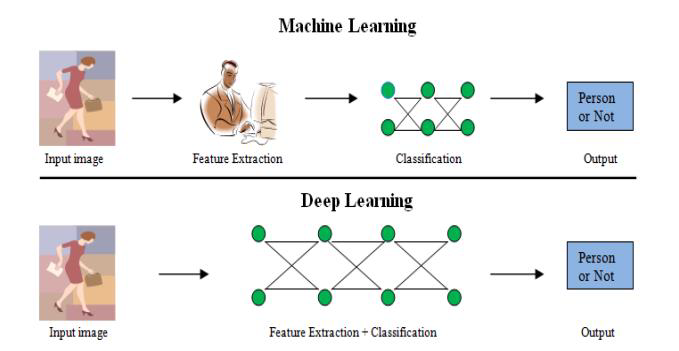
\includegraphics[width=0.8\textwidth]{img/2-Antecedentes/2.1-Estado_arte/ML_vs_DL.png}
    \caption{Machine Learning vs Deep Learning \cite{gupta2022deep}}
    \label{fig:2.1-ML_vs_DL}
\end{figure}

\par La detección de fallas en correas transportadoras se aborda como un problema de detección de objetos mediante aprendizaje supervisado. Existen dos enfoques principales: los modelos de dos etapas, como la familia R-CNN (red neuronal convolucional basada en regiones), que emplean redes de propuestas regionales seguidas de refinamiento, y los modelos de una etapa, como YOLO y SSD, que realizan predicciones por regresión directa, optimizados para aplicaciones en tiempo real \cite{zhang2021deep}. \\

\par La detección de objetos ha sido uno de los problemas centrales en visión por computadora, tradicionalmente abordado mediante arquitecturas basadas en redes neuronales convolucionales (CNN). Estos modelos dominaron el campo durante más de una década, impulsando desarrollos significativos en precisión y eficiencia. Sin embargo, alcanzar un balance óptimo entre velocidad y exactitud ha requerido explorar estructuras más allá del marco convencional de las CNN. Los modelos basados en transformers, originalmente desarrollados para procesamiento de lenguaje natural (Natural Language Processing), han demostrado ser altamente efectivos al capturar relaciones espaciales globales en imágenes, lo que los convierte en una propuesta a considerar para la implementación de nuevos modelos de detección de objetos \cite{arkin2023survey}. \\

\par Una memoria de título desarrollada en la Universidad de Chile \cite{angulo2024deteccion} implementa visión computacional y técnicas de aprendizaje profundo (Deep Learning) para la detección temprana de fallas en correas transportadoras, utilizando una de las versiones del modelo YOLO (You Only Look Once). El estudio describe detalladamente la implementación y calibración del modelo, además de proporcionar información técnica sobre redes neuronales convolucionales, métricas de evaluación, pruebas experimentales y resultados ilustrativos.

%%%%%%%%%%%%%%%%%%%%%%%%%%%%%%%%%%%%%%%%%%%%%%%
\subsection{Fallas en correas transportadoras}

\par Las correas transportadoras operan en condiciones que las exponen a diversos tipos de daños, los cuales pueden generar costosos tiempos de inactividad. Para cada condición de falla, se han revisado exhaustivamente sus tipos y causas, así como los métodos adecuados para su mitigación, contribuyendo a mejorar la confiabilidad del sistema \cite{khanna2022types}. \\

\par Entre las fallas más comunes en correas transportadoras se identifican el \textbf{daño por impacto}, que puede provocar \textbf{perforaciones o roturas locales}; la \textbf{delaminación}, generada por esfuerzos cíclicos y fatiga; y la \textbf{desalineación de la banda}, que causa \textbf{desgaste anómalo en los bordes}. Además, se reporta \textbf{desgaste abrasivo} en la cubierta superior por efecto de partículas duras, \textbf{rotura de cables de acero} en correas reforzadas, y \textbf{cortes longitudinales y transversales}, todos los cuales afectan directamente la vida útil y seguridad operativa del sistema.


\begin{figure}[H]
    \centering
    \subfloat[Desgasta abrasivo banda]{
        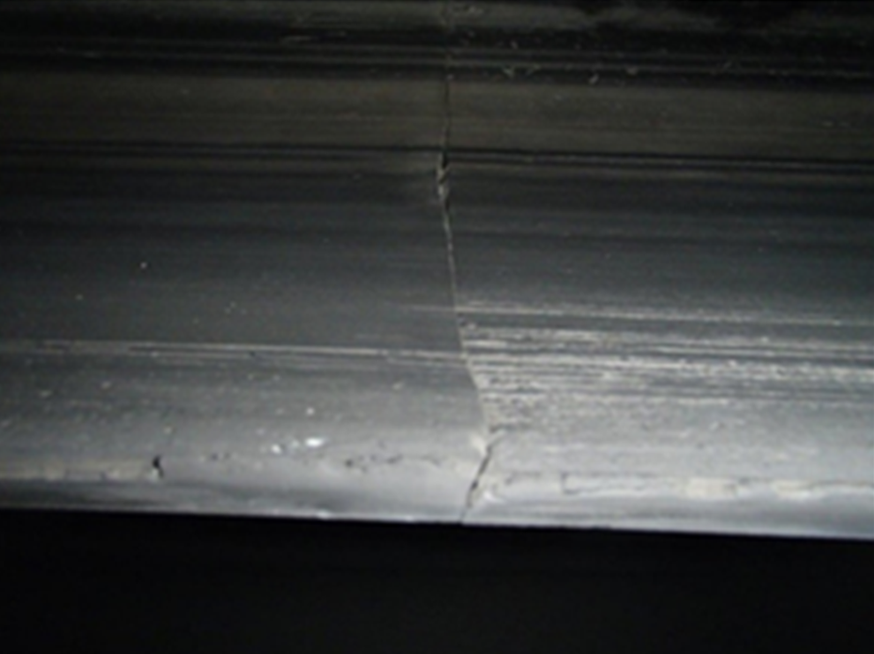
\includegraphics[width=0.23\textwidth]{img/2-Antecedentes/Fotos_Fallas/Desgaste_abrasivo_banda.png}
    }
    \hfill
    \subfloat[Desgaste abrasivo bordes banda]{
        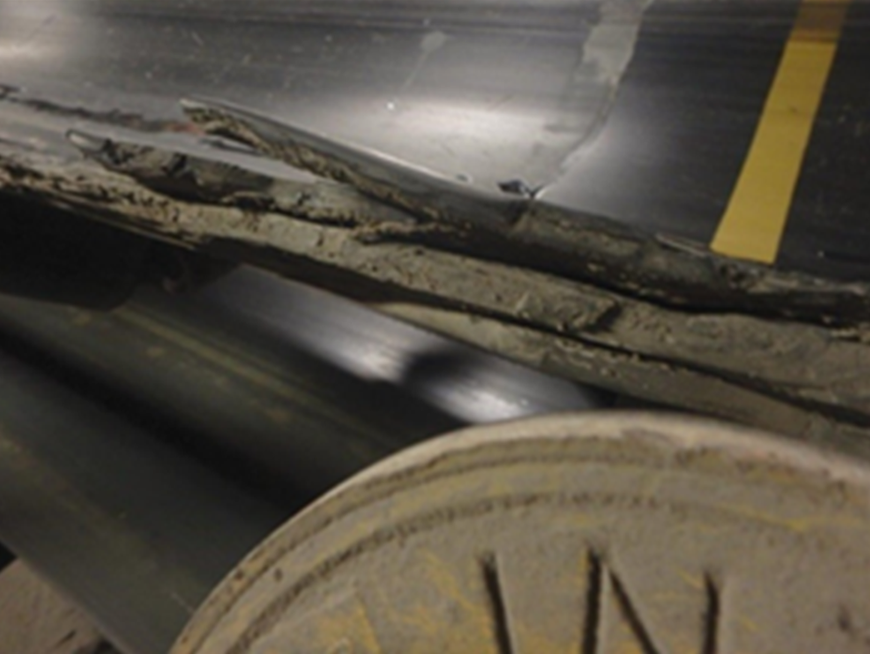
\includegraphics[width=0.23\textwidth]{img/2-Antecedentes/Fotos_Fallas/Desgaste_abrasivo_banda_bordes.png}
    }
    \hfill
    \subfloat[Perforación de banda]{
        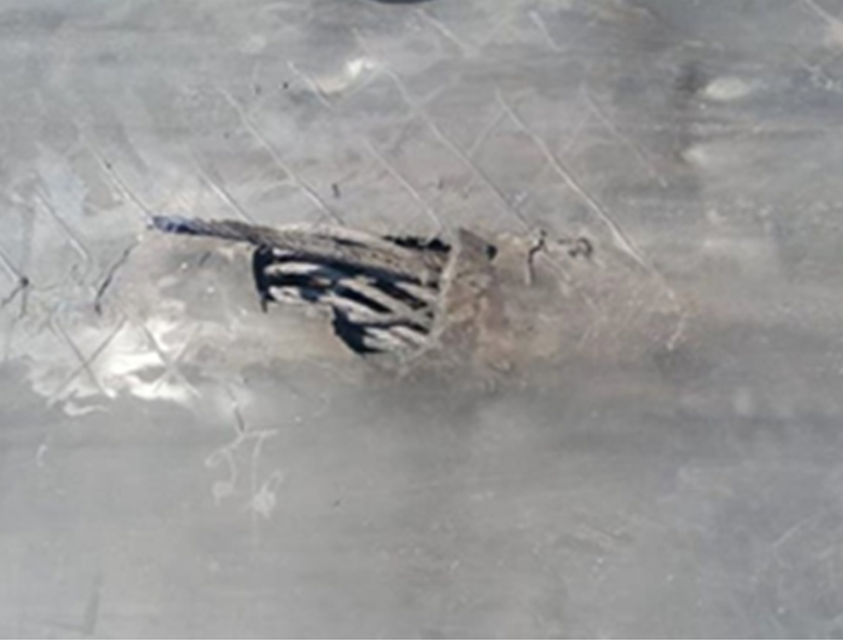
\includegraphics[width=0.23\textwidth]{img/2-Antecedentes/Fotos_Fallas/Perforacion_banda.png}
    }
    \hfill
    \subfloat[Rotura de banda]{
        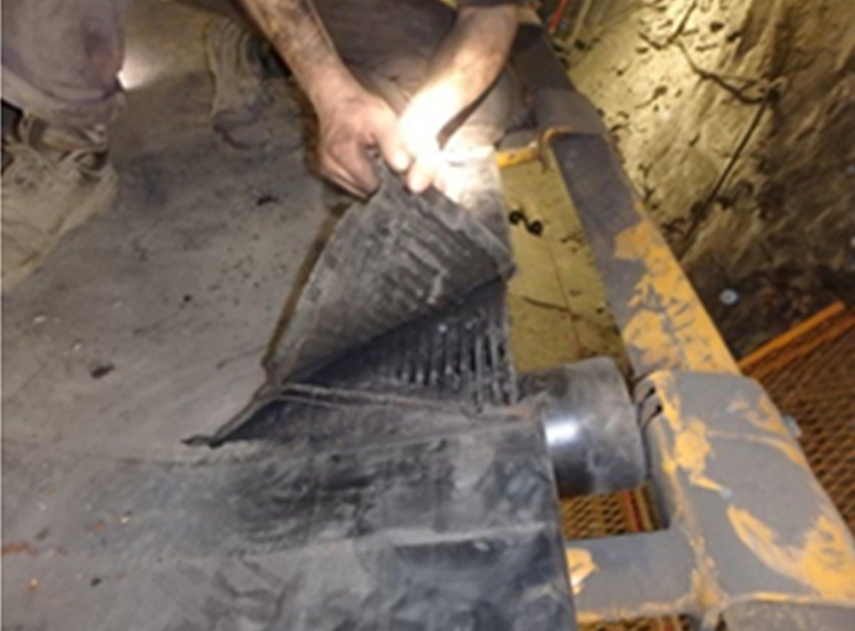
\includegraphics[width=0.23\textwidth]{img/2-Antecedentes/Fotos_Fallas/Rotura_banda.png}
    }
    \hfill
    \subfloat[Corte longitudinal ó Desgarro]{
        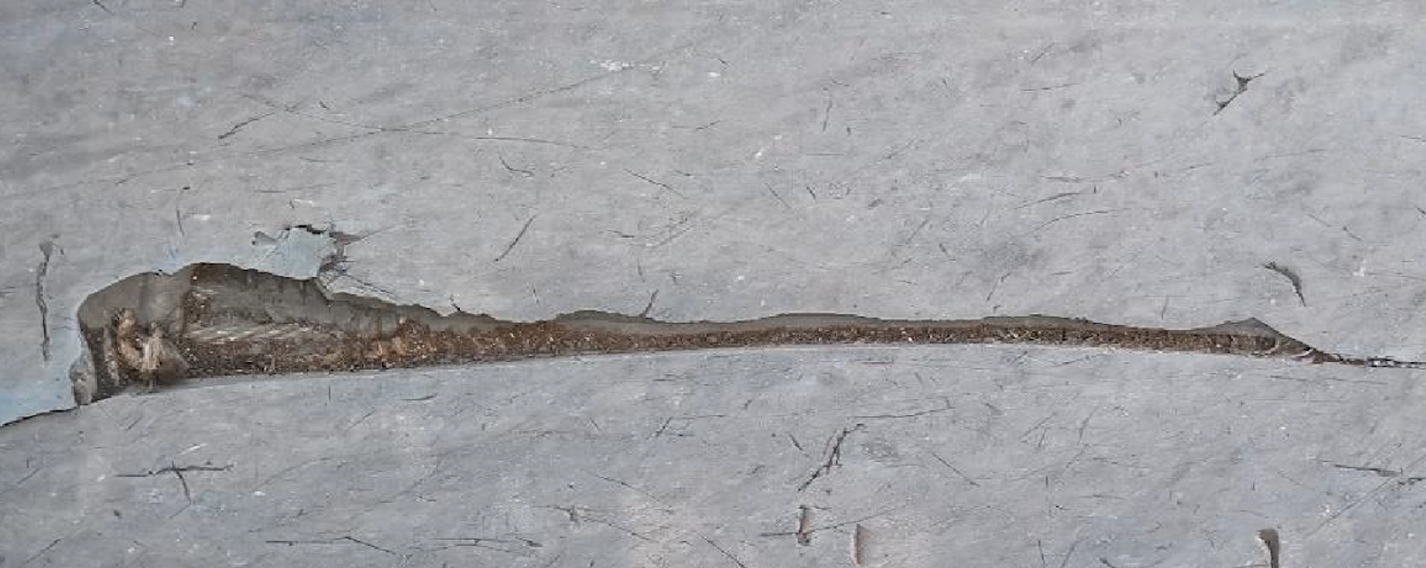
\includegraphics[width=0.4\textwidth]{img/2-Antecedentes/Fotos_Fallas/Corte_longitudinal.png}
    }
    \caption{Tipos de falla comunes en correas transportadoras, imágenes adaptadas de \cite{khanna2022types}.}
    \label{fig:falla_correas}
\end{figure}
%%%%%%%%%%%%%%%%%%%%%%%%%%%%%%%%%%%%%%%%%%%%%%%%%

\section{Redes Neuronales Convolucionales (CNN)}

\subsection{Arquitectura}

\par La detección de objetos en visión por computadora consiste en identificar automáticamente instancias u objetos presentes en una imagen o secuencia, localizándolos mediante cajas delimitadoras y asignándoles una clase. En los modelos modernos, esta tarea se formula como un problema conjunto de clasificación y regresión: para cada región candidata de la imagen se predice la probabilidad de pertenencia a una clase y las coordenadas de la caja delimitadora asociada. Para abordar este problema de manera eficiente, las arquitecturas actuales separan conceptualmente el modelo en dos bloques: (i) un \textit{backbone} convolucional que extrae mapas de características jerárquicos desde la imagen de entrada y (ii) una o varias cabezas de detección encargadas de proyectar dichos mapas en predicciones de clases y cajas delimitadoras \cite{kaur2022tools,lubinus2023redes}. \\

\begin{figure}[H]
    \centering
    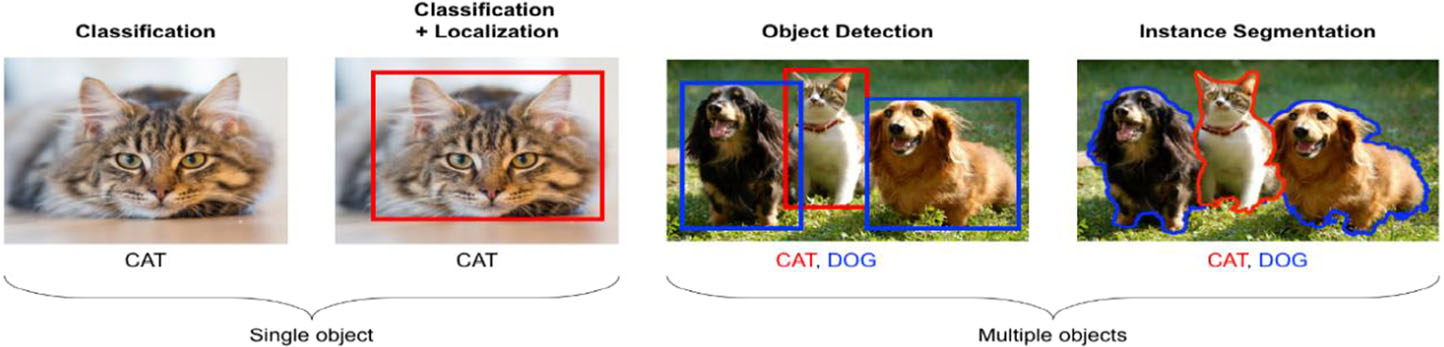
\includegraphics[width=0.9\textwidth]{img/2-Antecedentes/2-Object_Detection_example.png}
    \caption{Ejemplos de detección de objetos simples y múltiples. Imagen adaptada de \cite{kaur2022tools}.}
    \label{fig:2.2-object_detection_example}
\end{figure}

\par En este contexto, las redes neuronales convolucionales (CNN) constituyen el núcleo de la mayoría de arquitecturas de visión por computador. Una CNN está formada por una sucesión de capas de convolución, funciones de activación no lineales (como ReLU o variantes), capas de normalización y, en algunos casos, capas de reducción de dimensionalidad (\textit{pooling}). Las convoluciones aplican filtros o \textit{kernels} que se desplazan sobre la imagen, compartiendo pesos en el plano espacial. Este mecanismo reduce el número de parámetros, explota la estructura local de las imágenes y confiere invariancia aproximada a traslaciones \cite{lubinus2023redes}. \\

\par Tal como se describe en revisiones recientes de aprendizaje profundo, las primeras capas de una CNN tienden a aprender características de bajo nivel (bordes, texturas, gradientes de intensidad), mientras que las capas intermedias y profundas capturan patrones de mayor complejidad (formas, partes de objetos y, finalmente, representaciones semánticas de alto nivel). Este aprendizaje jerárquico permite que una misma arquitectura pueda generalizar sobre grandes volúmenes de datos y adaptarse a distintas tareas visuales mediante el ajuste de sus parámetros \cite{gupta2022deep,lubinus2023redes}. \\

\par En las capas de reducción o \textit{pooling}, como el \textit{max pooling}, se disminuye la resolución espacial de los mapas de características conservando las activaciones más relevantes. Esta etapa reduce la carga computacional y actúa como un mecanismo de regularización, al atenuar pequeños desplazamientos o deformaciones locales en la imagen. Finalmente, uno o varios bloques de capas densas (\textit{fully connected}) agregan la información extraída y realizan la clasificación o regresión final, según el diseño del modelo \cite{lubinus2023redes}. \\

\par Para tareas de detección de objetos, las CNN se integran habitualmente en una arquitectura de tipo \textit{backbone--neck--head}. El \textit{backbone} (por ejemplo, variantes de VGG, ResNet u otras arquitecturas optimizadas para eficiencia) extrae los mapas de características base. Sobre estos mapas, el \textit{neck} construye representaciones multiescala mediante estructuras como pirámides de características (FPN, PAN), lo que permite detectar objetos de distintos tamaños. Finalmente, la \textit{head} de detección proyecta esas características a predicciones de clases y cajas delimitadoras, como ocurre en los modelos de una sola etapa (\textit{single-shot}) tipo YOLO y SSD, descritos en secciones posteriores \cite{zhang2021deep}. \\

\subsection{Hiperparámetros comunes}

\par Las arquitecturas basadas en CNN dependen de un conjunto de hiperparámetros que controlan tanto la forma de la red como el proceso de entrenamiento. A diferencia de los parámetros internos del modelo (pesos y sesgos), los hiperparámetros se fijan externamente y condicionan la calidad de las representaciones aprendidas, la velocidad de convergencia y el grado de generalización. En aplicaciones de detección de objetos, la adecuada configuración de estos hiperparámetros resulta crítica para lograr un equilibrio entre precisión y costo computacional \cite{gupta2022deep,zhang2021deep}. \\

\par En la práctica, muchos de estos hiperparámetros son compartidos por distintas arquitecturas de detección basadas en CNN (por ejemplo, SSD, YOLO o variantes híbridas), lo que permite definir configuraciones iniciales razonables y posteriormente ajustarlas de forma iterativa. La Tabla \ref{tab:2-hiperparametros-comunes-cnn} resume algunos de los hiperparámetros más habituales, junto con rangos típicos y una descripción de su efecto sobre el entrenamiento del modelo. \\

\begin{table}[H]
    \centering
    \caption{Hiperparámetros comunes en modelos de detección basados en CNN}
    \begin{tabular}{|c|c|c|}
        \hline
        \textbf{Hiperparámetro} & \textbf{Rango típico} & \textbf{Nombre} \\ 
        \hline
        $lr0$ & $10^{-5}$ -- $10^{-1}$ & Tasa de aprendizaje inicial \\ 
        \hline
        $lrf$ & 0,01 -- 1,0 & Factor de tasa final \\ 
        \hline
        Número de \textit{épocas} & 100 -- 150 & \textit{Épocas} de entrenamiento \\ 
        \hline
        Tamaño de imagen & $640 \times 640$ píxeles & Resolución de entrada \\ 
        \hline
        Tamaño de \textit{batch} & 4 / 8 / 16 imágenes & Tamaño de lote (\textit{batch}) \\ 
        \hline
        $weight\_decay$ & 0,0 -- 0,001 & Regularización $L_2$ \\ 
        \hline
        $box\_loss$ & 0,02 -- 0,2 & Peso pérdida de cajas \\ 
        \hline
        $cls\_loss$ & 0,02 -- 4,0 & Peso pérdida de clasificación \\ 
        \hline
        $object\_loss$ & 0,02 -- 0,04 & Peso pérdida de objeto \\ 
        \hline
        $warmup\_epochs$ & 0 -- 5 & \textit{Épocas} de calentamiento \\ 
        \hline
    \end{tabular}
    \label{tab:2-hiperparametros-comunes-cnn}
\end{table}





%%%%%%%%%%%%%%%%%%%%%%%%%%%%%%%%%%%%%%%%%%%%%%%
\section{Mecanismo de atención y arquitectura Encoder-Decoder}

\subsection{Mecanismo de atención en transformers}

\par Los modelos modernos basados en transformers utilizan mecanismos de auto-atención para ponderar de manera dinámica la relevancia de cada elemento de la entrada con respecto a los demás. En el contexto de visión por computador, la imagen se representa como una secuencia de \textit{tokens} (por ejemplo, parches proyectados a un espacio de embeddings), sobre los cuales la auto-atención estima qué regiones resultan más informativas para la tarea. Este esquema permite capturar dependencias espaciales de largo alcance, superando la limitación local de los filtros convolucionales clásicos. \\

\par Debido a la complejidad de estos mecanismos, han surgido métodos de explicabilidad que permiten visualizar la contribución de cada token de entrada en la inferencia. Entre ellos, se propone un enfoque general aplicable a arquitecturas bi-modales y encoder-decoder, capaz de generar mapas de atención interpretables a partir de las ponderaciones internas del modelo. Estas herramientas de interpretabilidad resultan especialmente útiles en arquitecturas de detección basadas en transformers, donde la distribución de la atención sobre la imagen entrega información complementaria sobre las regiones que influyen en la predicción final \cite{chefer2021generic}. \\

\subsection{Arquitecturas encoder-decoder para detección de objetos}

\par En tareas de detección de objetos, los transformers suelen organizarse bajo un esquema encoder-decoder. Modelos como DETR y DINO utilizan un codificador (\textit{encoder}) que transforma la imagen en una representación latente mediante auto-atención, y un decodificador (\textit{decoder}) que cruza estas representaciones con un conjunto fijo de consultas (\textit{object queries}) para predecir directamente las clases y localizaciones de los objetos presentes. De este modo, el problema de detección se formula como un mapeo directo entre un conjunto de consultas y las instancias de objetos en la imagen, evitando componentes manuales como los algoritmos de propuestas de regiones \cite{carion2020end,zhang2022dino}. \\

\par En versiones más recientes, como DINO, se introducen mejoras sobre el esquema original de DETR mediante el uso de extractores de características multiescala, atención deformable y estrategias de entrenamiento con ramas de desruido (\textit{denoising}). Estas extensiones permiten una convergencia más rápida y una gestión más robusta de muestras difíciles, manteniendo la formulación encoder-decoder como eje central de la arquitectura \cite{zhang2022dino}. \\

\par De manera complementaria, la destilación de conocimiento (\textit{knowledge distillation}) se ha incorporado como una estrategia para transferir la capacidad representacional de modelos visuales de gran escala (\textit{teacher}) hacia arquitecturas más livianas y eficientes (\textit{student}). En el contexto de la detección de objetos con transformers, esta técnica permite condensar el conocimiento aprendido por modelos preentrenados en clasificación o detección sobre grandes bases de datos, reduciendo el costo computacional en la inferencia sin sacrificar significativamente el rendimiento \cite{li2024distilling}. \\




%%%%%%%%%%%%%%%%%%%%%%%%%%%%%%%%%%%%%%%%%%%%%%%
\clearpage
\section{Modelos de detección de objetos de una sola etapa (YOLO y SSD)}


\subsection{Contextualización}


\par YOLO y SSD pertenecen a la familia de modelos de detección de objetos de una sola etapa (\textit{one-stage detectors}), en los cuales la localización de las cajas delimitadoras y la clasificación de las instancias se realizan en una única pasada por la red. Ambos se basan en redes neuronales convolucionales (CNN) y se enmarcan dentro de los enfoques de detección de objetos con aprendizaje profundo (\textit{Deep Learning}), donde la propia red efectúa de manera conjunta la extracción de características y la predicción final. En la Figura~\ref{fig:2.4-YOLO_SSD_DL} se esquematiza la relación entre los esquemas tradicionales de detección de objetos basados en \textit{Machine Learning}, los modelos de una etapa como YOLO y SSD —que serán objeto de estudio en esta memoria— y los modelos de dos etapas (\textit{two-stage}), dentro de los cuales destaca la familia R-CNN, pionera en el uso de propuestas de regiones como base para la extracción de características y la detección posterior \cite{kaur2022tools}. \\

\begin{figure}[H]
    \centering
    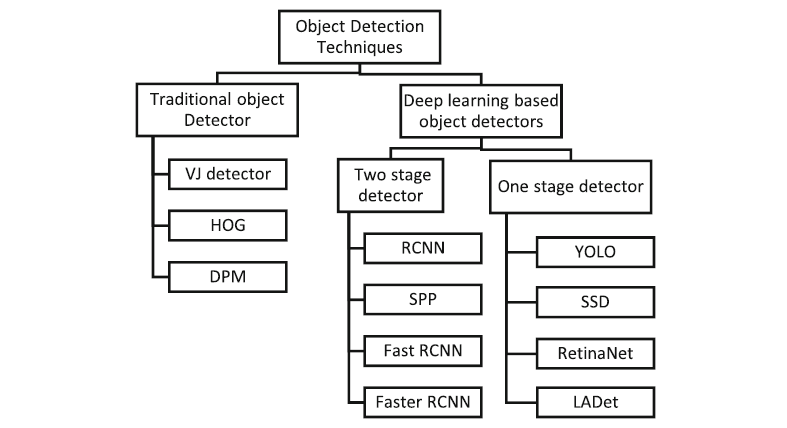
\includegraphics[width=0.8\textwidth]{img/2-Antecedentes/2.4-YOLO_SSD/YOLO_SSD_DL.png}
    \caption{Clasificación de varias técnicas de detección de objetos. Imagen extraída de \cite{kaur2022tools}.}
    \label{fig:2.4-YOLO_SSD_DL}
\end{figure}



\subsection{YOLO (You Only Look Once)}

\par YOLO (You Only Look Once) es un enfoque de detección de objetos de una sola etapa que destaca por su alta velocidad y eficiencia, al predecir directamente las clases y ubicaciones de objetos en una sola pasada por la red. A diferencia de métodos de dos etapas como R-CNN o Faster R-CNN, YOLO evita la generación de propuestas de regiones, lo que lo hace apto para aplicaciones en tiempo real. Su arquitectura unificada lo convierte en una opción balanceada entre precisión y velocidad \cite{terven2023comprehensive}.\\

\par 

\begin{figure}[H]
    \centering
    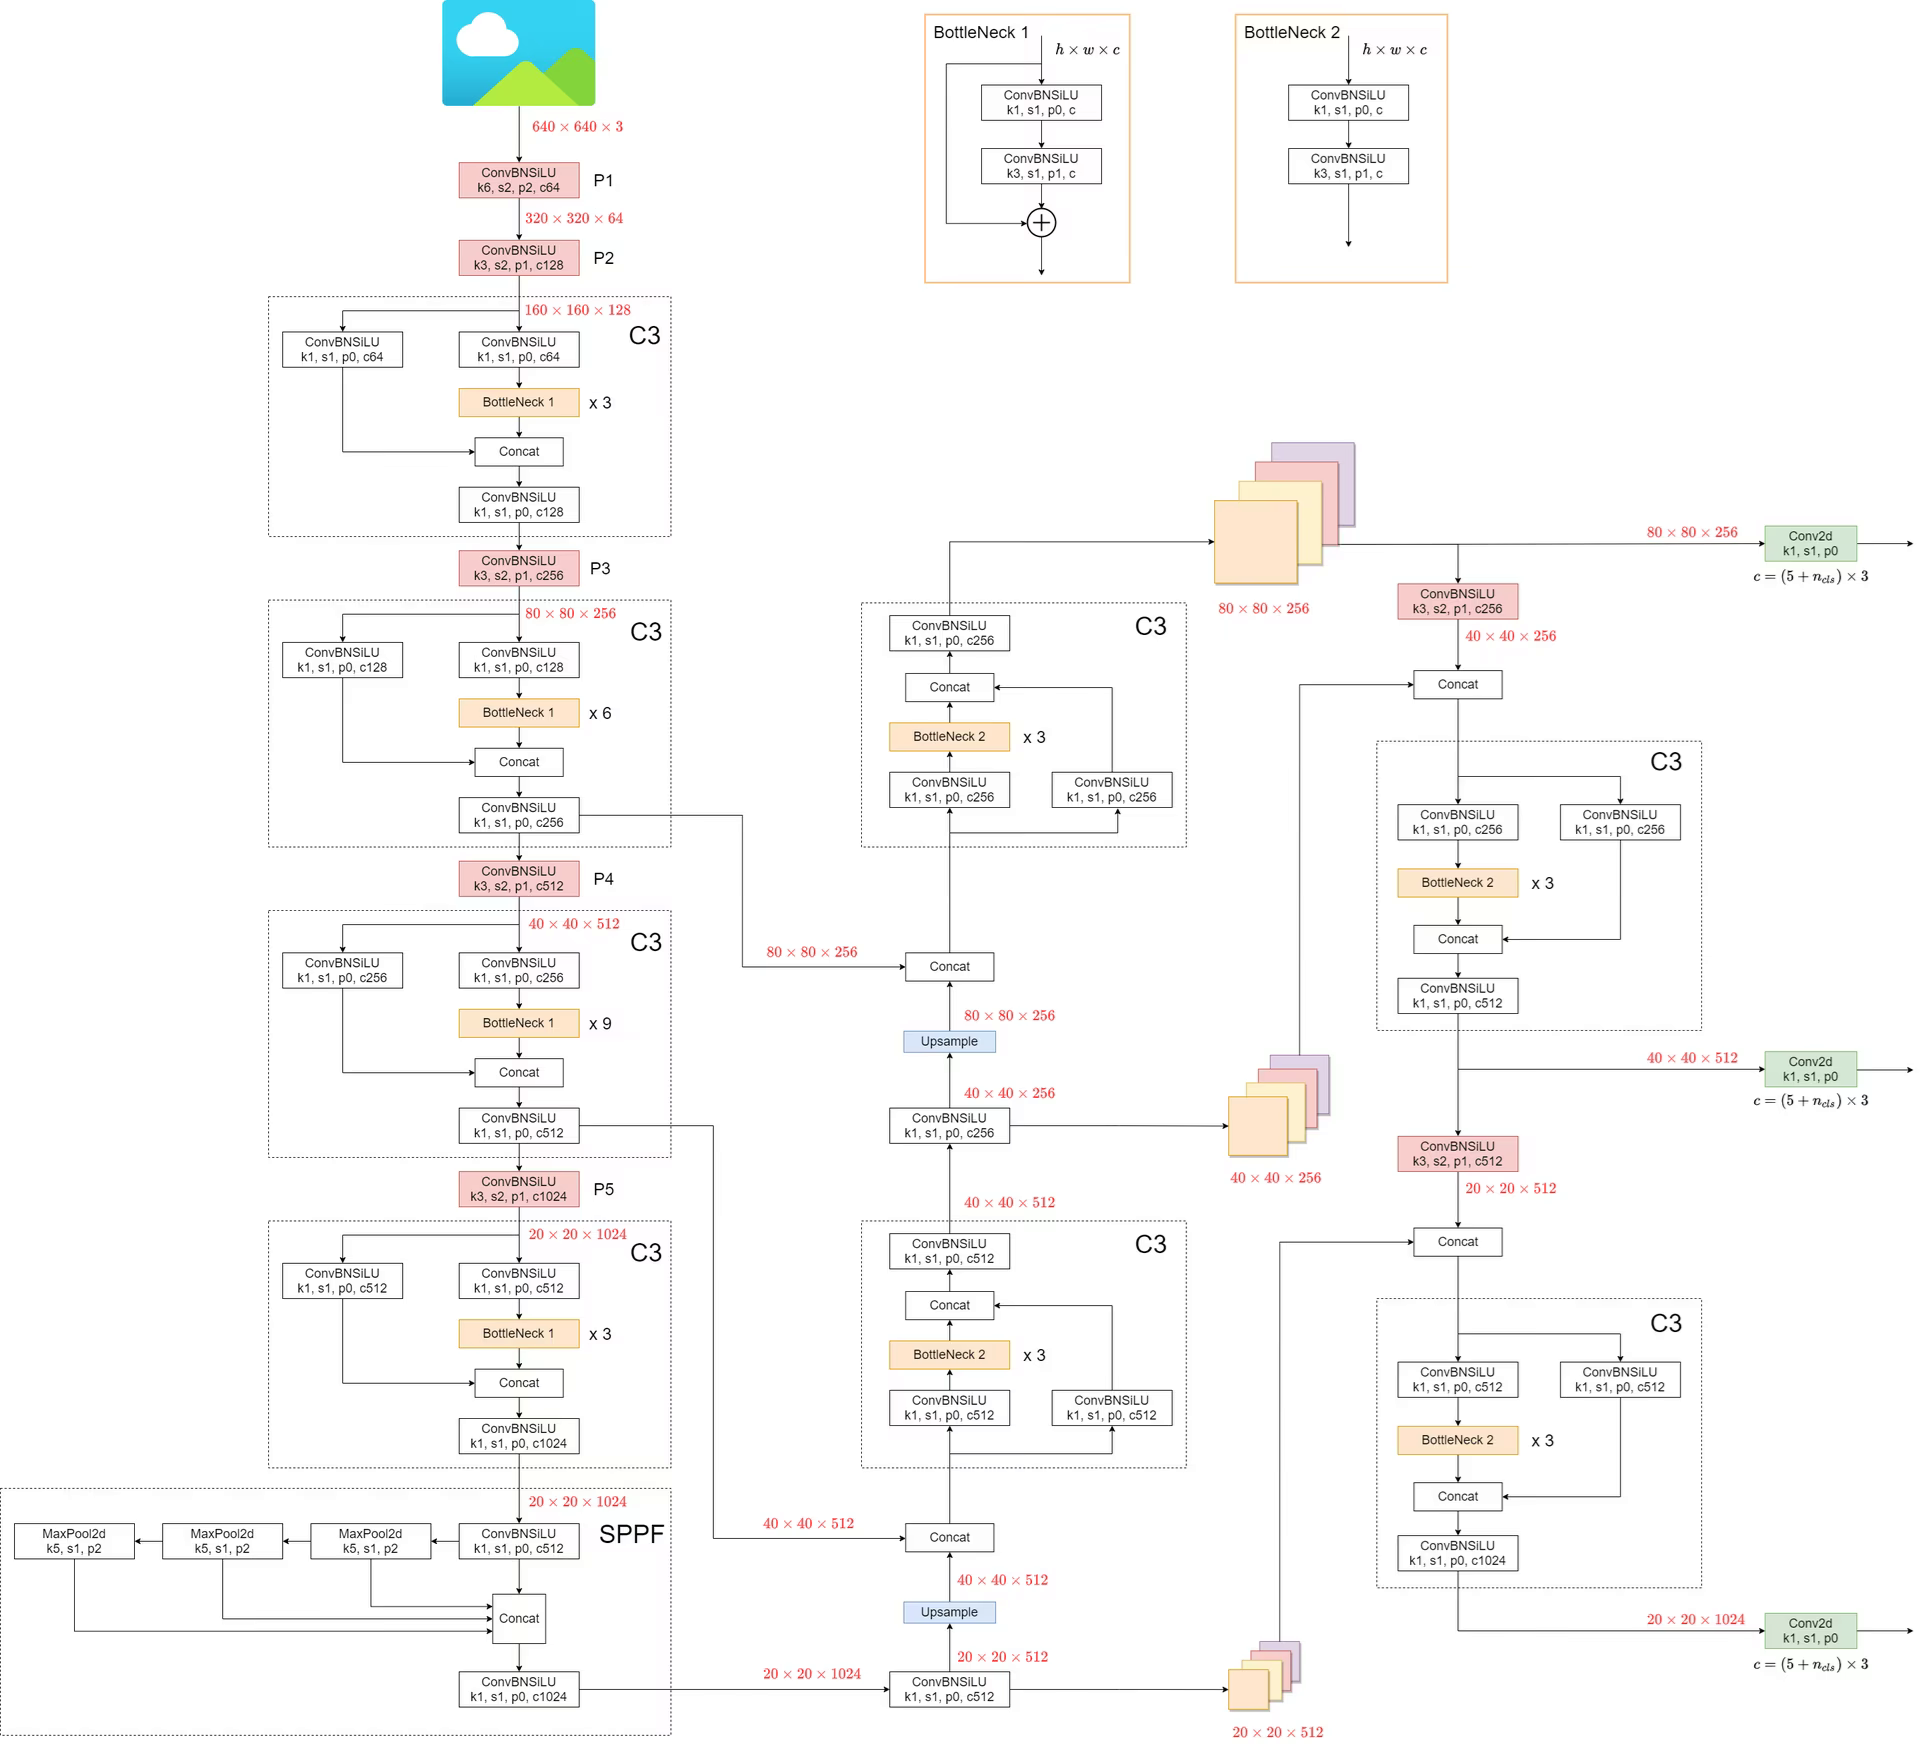
\includegraphics[width=0.9\textwidth]{img/2-Antecedentes/2.4-YOLO_SSD/YOLO_v5_Architecture_l.png}
    \caption{Arquitectura de YOLOv5.}
    \label{fig:2.4-YOLO_v5_architecture}
\end{figure}



\subsection{SSD (Single Shot Multibox Detector)}

\par SSD (Single Shot Multibox Detector) es otro enfoque en la detección de objetos, caracterizado por su capacidad de realizar clasificación y regresión de cajas delimitadoras en una única pasada de la red, sin requerir etapas de propuesta de regiones. SSD utiliza múltiples mapas de características de diferentes escalas para detectar objetos de diversos tamaños, lo que mejora la precisión especialmente en objetos pequeños \cite{liu2016ssd}. La arquitectura general (que contempla sus dos versiones), se muestra en la Figura \ref{fig:2.4-SSD_architecture}.
  
\begin{figure}[H]
    \centering
    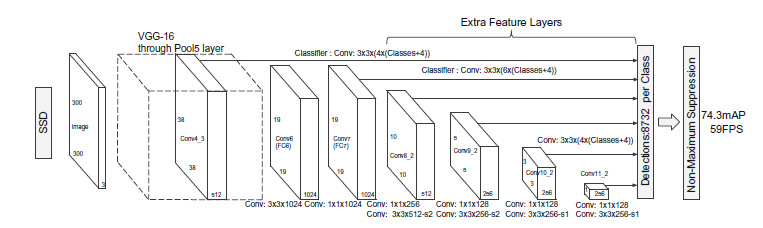
\includegraphics[width=0.8\textwidth]{img/2-Antecedentes/2.4-YOLO_SSD/SSD_Architecture.png}
    \caption{Arquitectura general de SSD. Imagen extraída y procesada de \cite{liu2016ssd}.}
    \label{fig:2.4-SSD_architecture}
\end{figure}

\par 

\subsection{Hiperparámetros}

\par Los hiperparámetros son valores que controlan el proceso de aprendizaje y condicionan los parámetros internos que el modelo ajusta durante el entrenamiento. Se denominan así por encontrarse en un nivel superior, ya que no forman parte del modelo aprendido, sino que guían su optimización. Al finalizar el entrenamiento, el modelo resultante contiene únicamente los parámetros ajustados, mientras que los hiperparámetros utilizados permanecen externos a dicha estructura \cite{nyuytiymbiy2020parameters}.
\\

\par El ajuste de hiperparámetros en los modelos de detección de objetos basados en redes neuronales convolucionales, es un proceso iterativo el cual está destinado a optimizar las métricas de evaluación utilizadas en visión computacional \cite{ultralytics2025hyperparam}.


%%%%%%%%%%%%%%%%%%%%%%%%%%%%%%%%%%%%%%%%%%%%%%%
\section{DETR (DEtection TRansformer) y DINO}

\subsection{Arquitecturas}

\par DETR y DINO son modelos de detección de objetos basados en la arquitectura de transformers, originalmente desarrollada para procesamiento de lenguaje natural, pero adaptada para visión por computadora. 
\\

%DETR
\par DETR (DEtection TRansformer) es un modelo de aprendizaje profundo (deep-learning), compuesta por tres elementos principales: un backbone convolucional (CNN backbone) que extrae las representaciones visuales, un transformador encoder-decoder (encoder-decoder transformer) que modela relaciones globales en la imagen, y una red neuronal completamente conectada (feed forward network, FFN) que realiza las predicciones finales. DETR no requiere componentes manuales ni estructuras complejas, lo que permite su implementación en frameworks de aprendizaje profundo estándar con pocas líneas de código \cite{carion2020end}. \\

%DINO

\par DINO es un modelo basado en DETR que incluye un backbone, un encoder y decoder multi-capa de Transformer, y múltiples cabezas de predicción (prediction heads). Emplea extractores de características multiescala que se procesan con embeddings posicionales (positional embeddings) en el encoder. Su innovación principal. respecto a DETR, es la selección mixta de queries (solicitudes) para inicializar anclas posicionales (positional anchors) en el decoder, mientras que las queries de contenido (content queries) permanecen aprendibles. Utiliza atención deformable (deformable attention) para actualizar características capa a capa y cuenta con una rama de desruido (denoising) con entrenamiento contrastivo, mejorando la gestión de muestras difíciles \cite{zhang2022dino}.



\subsection{Hiperparámetros}

\par En el modelo DETR, los hiperparámetros incluyen configuraciones específicas del número de \textit{layers} (capas) en la arquitectura, tasas de \textit{regularization} (regularización), tipo de \textit{optimizer} (optimizador) y esquemas de \textit{data augmentation} (aumento de datos) \cite{carion2020end}.
\\

\par En el modelo DINO, los hiperparámetros comparten similitudes con DETR, incluyendo el uso del optimizador AdamW con regularización por decaimiento de peso (weight decay) y ajustes en la tasa de aprendizaje mediante un programador dinámico (learning rate scheduler). Además, DINO incorpora un conjunto fijo y ampliado de consultas para el decoder (decoder queries), optimizando el equilibrio entre desempeño y costo computacional durante el entrenamiento \cite{zhang2022dino}.
%%%%%%%%%%%%%%%%%%%%%%%%%%%%%%%%%%%%%%%%%%%%%%
\section{Métricas}

\par Con el fin de validar la implementación de los modelos de detección de objetos para la clasificación de fallas, se emplean métricas cuantitativas estándar en visión por computador. El uso de estas métricas otorgan las herramientas esenciales para evaluar críticamente y de forma fiable los modelos implementados \cite{schlosser2024overview}.

\subsection{Precisión, Exhaustividad y F-Score}

\par La \textbf{precisión} (\textit{precision}) mide la proporción de verdaderos positivos entre todas las predicciones positivas. El \textbf{recall} o \textit{exhaustividad} mide la proporción de verdaderos positivos detectados sobre los positivos reales. 

\[
\text{Precision} = \frac{TP}{TP + FP} \quad \quad \text{Recall} = \frac{TP}{TP + FN}
\]

\begin{table}[H]
    \centering
    \begin{tabular}{|c|c|}
        \hline
         \textbf{Abreviación} & \textbf{Significado}  \\
         \hline
         T & Total \\
         \hline
         P & Positivos \\
         \hline
         N & Negativos \\
         \hline
         TP & Verdaderos Positivos \\
         \hline
         TN & Verdaderos Negativos \\
         \hline
         FP & Falsos Negativos \\
         \hline
         n & Número de Clases \\
         \hline
    \end{tabular}
    \caption{Definiciones generales \textit{Machine Learning} \cite{schlosser2024overview}}
    \label{tab:2-def_metricas}
\end{table}


\par El \textbf{F-Score} ($F_{\beta}$) es la media ponderada entre precisión y recall, ajustada por el parámetro $\beta$. Un caso particular es el \textbf{F1-Score} ($F_{1}$), donde $\beta = 1$.

\[
F_{\beta} = (1 + \beta^2) \cdot \frac{\text{Precision} \cdot \text{Recall}}{\beta^2 \cdot \text{Precision} + \text{Recall}} \quad \quad F_1 = 2 \cdot \frac{\text{Precision} \cdot \text{Recall}}{\text{Precision} + \text{Recall}}
\]

\subsection{IoU y Confianza}

\par El \textbf{IoU (Intersection over Union)} evalúa el solapamiento entre la predicción y la verdad de terreno:
\\
\[
\text{IoU} = \frac{\text{Área de Intersección}}{\text{Área de Unión}}
\]

\par La \textbf{confianza} asigna una probabilidad a la predicción, y el \textbf{umbral de confianza} define el valor mínimo para aceptar una detección.

\subsection{AP y mAP}

\par La \textbf{Average Precision (AP)} corresponde al área bajo la curva precisión-recall para una clase. El \textbf{mean Average Precision (mAP)} es el promedio del AP para todas las clases. \\

\par El \textbf{mAP@50} utiliza un umbral IoU fijo de 0{,}5. \textbf{mAP@50-95} promedia el AP en umbrales de IoU entre 0{,}5 y 0{,}95 (paso de 0{,}05), reflejando un criterio más exigente y robusto.

\subsection{Matriz de Confusión}

\par Representa los aciertos y errores del clasificador mediante los conteos de verdaderos/falsos positivos y negativos por clase, permitiendo un análisis detallado del comportamiento del modelo.
